\let\negmedspace\undefined
\let\negthickspace\undefined
\documentclass[journal,12pt,onecolumn]{IEEEtran}
\usepackage{cite}
\usepackage{amsmath,amssymb,amsfonts,amsthm}
\usepackage{algorithmic}
\usepackage{graphicx}

\graphicspath{{./figs/}}
\usepackage{textcomp}
\usepackage{xcolor}
\usepackage{txfonts}
\usepackage{listings}
\usepackage{enumitem}
\usepackage{mathtools}
\usepackage{gensymb}
\usepackage{comment}
\usepackage{caption}
\usepackage[breaklinks=true]{hyperref}
\usepackage{tkz-euclide}
\usepackage{gvv}
\usepackage[latin1]{inputenc}
\usepackage{xparse}
\usepackage{color}
\usepackage{array}
\usepackage{longtable}
\usepackage{calc}
\usepackage{multirow}
\usepackage{multicol}
\usepackage{hhline}
\usepackage{ifthen}
\usepackage{lscape}
\usepackage{tabularx}
\usepackage{array}
\usepackage{float}



\begin{document}

\title{2.5.29}
\author{EE25BTECH11061 - V.Sainadh}
{\let\newpage\relax\maketitle}

\textbf{Question:} 
The points $\vec{A} = (4,7),\ \vec{B} = (p,3),\ \vec{C} = (7,3)$ are the vertices of a right triangle, \\
right-angled at $\vec{B}$. Find the value of $p$.

\textbf{Solution: }Let
\begin{align}
\vec{A}=\myvec{4\\7},\quad
\vec{B}=\myvec{p\\3},\quad
\vec{C}=\myvec{7\\3}
\end{align}

Right angle at \(\vec{B}\) \(\implies\) the dot product of the adjacent sides at \(\vec{B}\) is zero:
\begin{align}
(\vec{A}-\vec{B})^T(\vec{C}-\vec{B})=0
\end{align}

Compute the vectors:
\begin{align}
\vec{A}-\vec{B}=\myvec{4-p\\4},\qquad
\vec{C}-\vec{B}=\myvec{7-p\\0}
\end{align}

Their dot product:
\begin{align}
(\vec{A}-\vec{B})^T(\vec{C}-\vec{B})
&= \myvec{4-p\\4}^T\myvec{7-p\\0} \\
&= (4-p)(7-p)+4\cdot 0 \\
&= (4-p)(7-p)
\end{align}
Right angle condition gives:
\begin{align}
(4-p)(7-p)=0 \ \Rightarrow\ p=4\ \text{or}\ p=7
\end{align}

If \(p=7\), then \(\vec{B}=\vec{C}\) (degenerate). Hence,
\begin{align}
\boxed{p=4}
\end{align}
\newpage

\textbf{Graph:}

\begin{figure}[H]
   \centering
   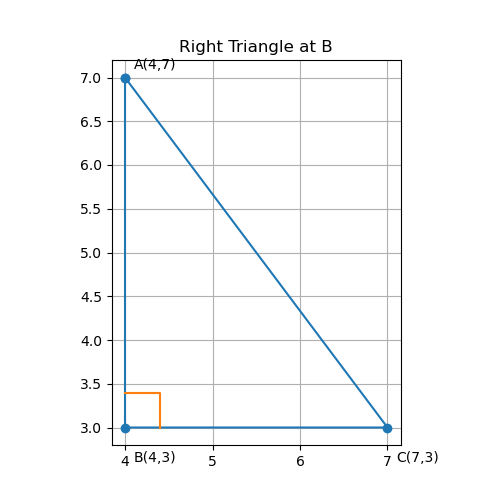
\includegraphics[width=0.8\columnwidth]{figs/Figure_1.png}
   \caption{Right Triangle at $\vec{B}$}
   \label{Plot_1}
\end{figure}


\end{document}
